\chapter{Introduction}\label{intro}
In this chapter discuss the decision of the proponents whether the research proposal turned out to be feasible or not. This study contains the information needed for deciding whether to proceed with creating the business. State the reasons why the proposed business could be considered feasible or not.

\section{Problem Statement}
Provide a one to two sentences introduction to this chapter. (Example: This chapter presents the market analysis and competitiveness of the proposed business.)
\begin{figure}
	\centering {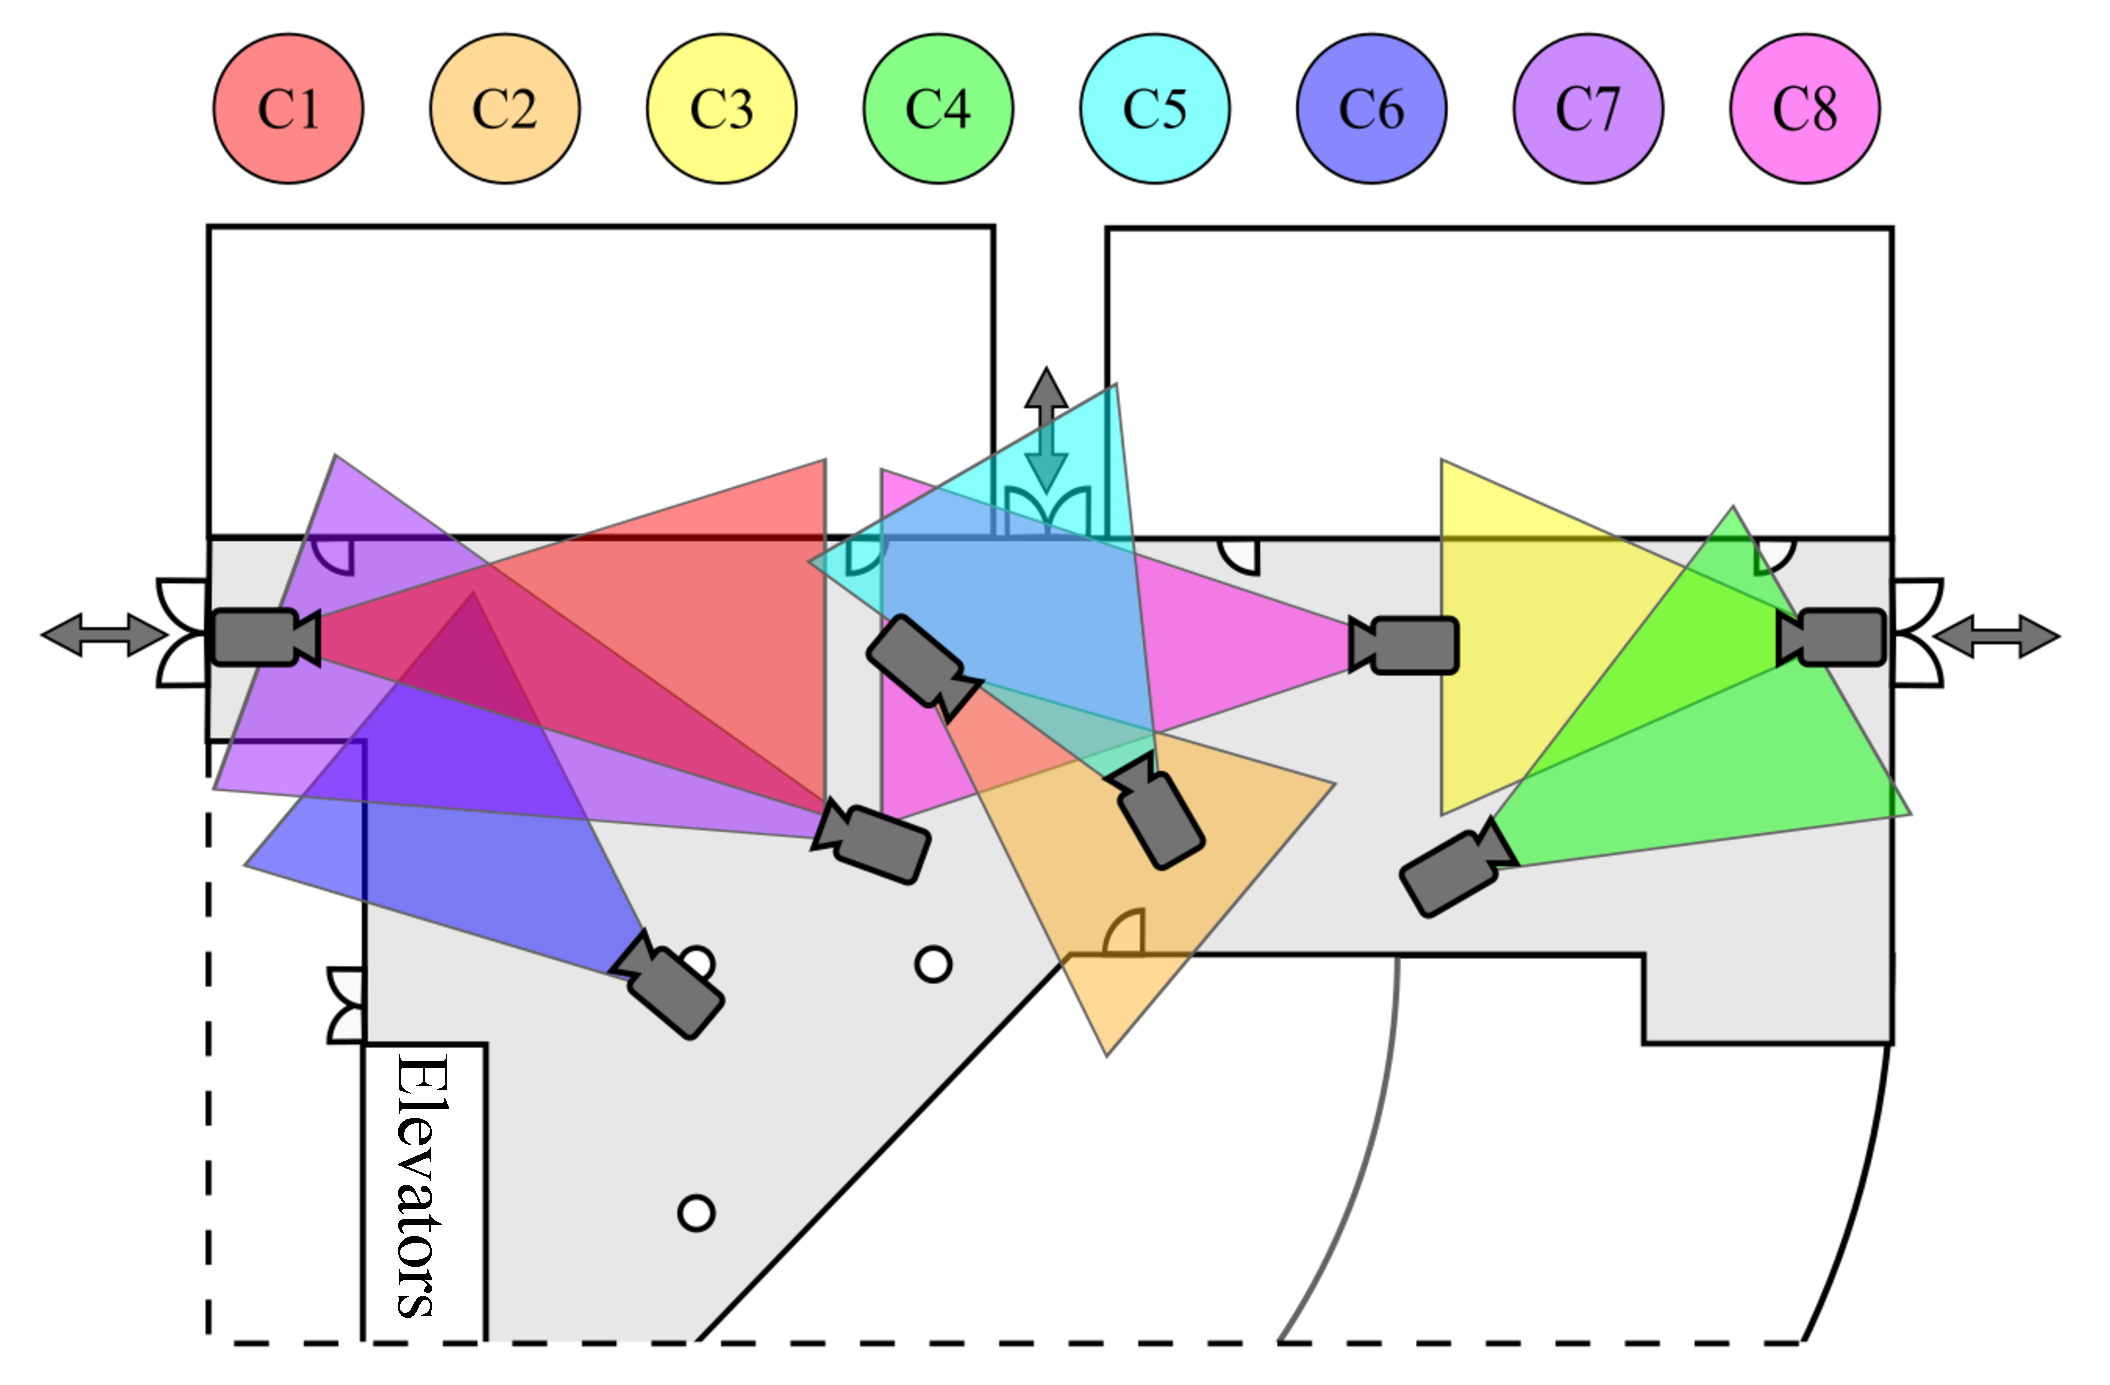
\includegraphics[width=0.7\textwidth]{figures/figure1.eps}}
	\caption
	{SEISD Lab \label{fig:example}}
\end{figure}


\section{Background}
From the proposal

\section{Benefits of Application} 
The rest of this thesis is organized as follows.

\section{Objectives} 
The rest of this thesis is organized as follows.

\section{Purpose} 
The rest of this thesis is organized as follows.

\section{Feature of Application} 
The rest of this thesis is organized as follows.

